%情報処理学会全国大会原稿テンプレート ver. 1.2

\documentclass[uplatex,twocolumn]{jsarticle}
\usepackage[top=30mm,bottom=25mm,left=20mm,right=20mm]{geometry}
\usepackage[T1]{fontenc}
\usepackage{txfonts}
\usepackage[expert,deluxe]{otf}
\usepackage[dvipdfmx,hiresbb]{graphicx}
\usepackage[dvipdfm]{hyperref}
\usepackage{pxjahyper}
\usepackage{multicol}
\setlength{\columnsep}{7mm}

\title{\vspace{-10mm}\Large{SNSにおいてフェイクニュースを拡散するユーザの特徴抽出}\footnotemark[0]}%要修正
\author{\large{岩橋 瑠伊\footnotemark[2]\qquad 矢吹 太朗}\\千葉工業大学 社会システム科学部 プロジェクトマネジメント学科\footnotemark[3]}%要修正
\date{}
\pagestyle{empty}
\begin{document}
\twocolumn[\maketitle]

\begingroup
\def\thefootnote{\fnsymbol{footnote}}
\footnotetext[0]{Feature extraction of users spreading fake news in SNS.}%要修正(最後はピリオド)
\footnotetext[2]{Rui Iwahashi (\verb|s1442014cr@s.chibakoudai.jp|)}%要修正
\footnotetext[3]{Department of Project Management, Faculty of Social Systems Science, Chiba Institute of Technology.}
\endgroup

\section{序論}
SNS上でフェイクニュースを拡散するユーザの特徴について調査する.SNSなどのウェブ上のメディアで,フェイクニュースが問題視されている\cite{dema1}.

例えば,2011年3月11日に発生した東日本大震災時に,携帯電話がつながらない状況下での有用な連絡手段として活躍した.しかし,その有用性はデマや誤情報も大量に拡散させる手助けとなりえる.実際に東日本大震災時に,数十種類のデマや誤情報が情報として拡散されてしまい,日本中を混乱させた.震災時のように連絡手段が限られた状況はこれからも発生する可能性は十分にあり,対策が必要である\cite{dema2}.

本研究では,デマが拡散されることを防ぐためにデマツイートをリツイートしているユーザの特徴抽出を行う.デマツイートがリツイートされる原因として,デマをデマと見抜けないユーザ,面白半分でリツイートしているユーザの2種類がいると考えた.この2種類のユーザと,それ以外のユーザにはTwitterの使い方に違いがあるのではないかと考えた.

\section{目的}
デマが拡散されることを防ぐために,デマツイートをリツイートしているユーザの特徴抽出を行う.そのために,現時点でデマだとわかっているツイートを過去に拡散したユーザの活動履歴を収集・分析する.分析結果をランダムサンプリングしたデータと比較することで,デマを拡散するようなユーザに共通する特徴を抽出し,その結果を報告する.

\section{手法}
デマツイートをリツイートするユーザーとそれ以外のユーザーの違いを見つけ,その違いが偶然生じたものではないことを示すために以下の手法で研究する.
\begin{enumerate}
\item ユーザIDを乱数で指定し,日本人ユーザ50人をランダムサンプリングする.
\item TwitterAPIを用いてデマツイートをリツイートしたユーザ50人を取得する.
\item TwitterAPIを用いて集めた各ユーザの最新100ツイートに含まれるリツイートの数を調べる.
\item 日本人ユーザ50人とデマツイートをリツイートしたユーザ50人の直近100ツイートに含まれるリツイートの数の平均の差が,偶然的な誤差の範囲にあるものかどうかを判断する為に2標本t検定を行う.
\end{enumerate}

\section{結果}
ユーザIDを乱数で指定し,日本人ユーザ50人をランダムサンプリングした.

以下の4つのデマツイートからそれぞれ50人のリツイートユーザを取得した.
\begin{itemize}
 \item デマツイート1として,ロンドンのテロ対策で有志のスパルタ兵が巡回しているというデマツイートがある.実際は映画の宣伝である.(TweetID:872255950131822596)
 \item デマツイート2として,国内のアリがヒアリに対抗出来るというデマツイートがある.実際は誤情報である.(TweetID:883170290242527232)
 \item デマツイート3として,PS4にPS2互換機能対応するというデマツイートがある.実際は誤情報である.(TweetID:882139486968205312)
 \item デマツイート4として,路上で乾燥海産物を売る人がいるが,それは麻酔薬で匂いを嗅いだら意識を失うというデマツイートがある.実際は昔韓国で流行したデマの内容と同じものである.(TweetID:923151745923948545)
\end{itemize}

ランダムサンプリングした日本人ユーザ50人の直近100ツイート中の平均リツイート数は20.04人,デマツイート1をリツイートしたユーザ50人の直近100ツイート中の平均リツイート数は56.68人,デマツイート2をリツイートしたユーザ50人の直近100ツイート中の平均リツイート数は62.64人,デマツイート3をリツイートしたユーザ50人の直近100ツイート中の58.46人となった,デマツイート4をリツイートしたユーザ50人の直近100ツイート中の平均リツイート数は57.92人となった.

デマツイート1と日本人ユーザ,デマツイート2と日本人ユーザ,デマツイート3と日本人ユーザ,デマツイート4と日本人ユーザのそれぞれ3組には対応がないデータなので,F検定を行い分散が等しいか等しくないかを確かめる.等分散の場合の2標本t検定と不等分散の場合のt検定をF検定の結果に沿って行った結果,全ての組み合わせで有意差が確認できた(有意水準は5%).

以下にデマツイート1~4をリツイートしたユーザの100ツイートあたりのリツイート数のヒストグラムを示す.

\begin{figure}[htbp]
\centering
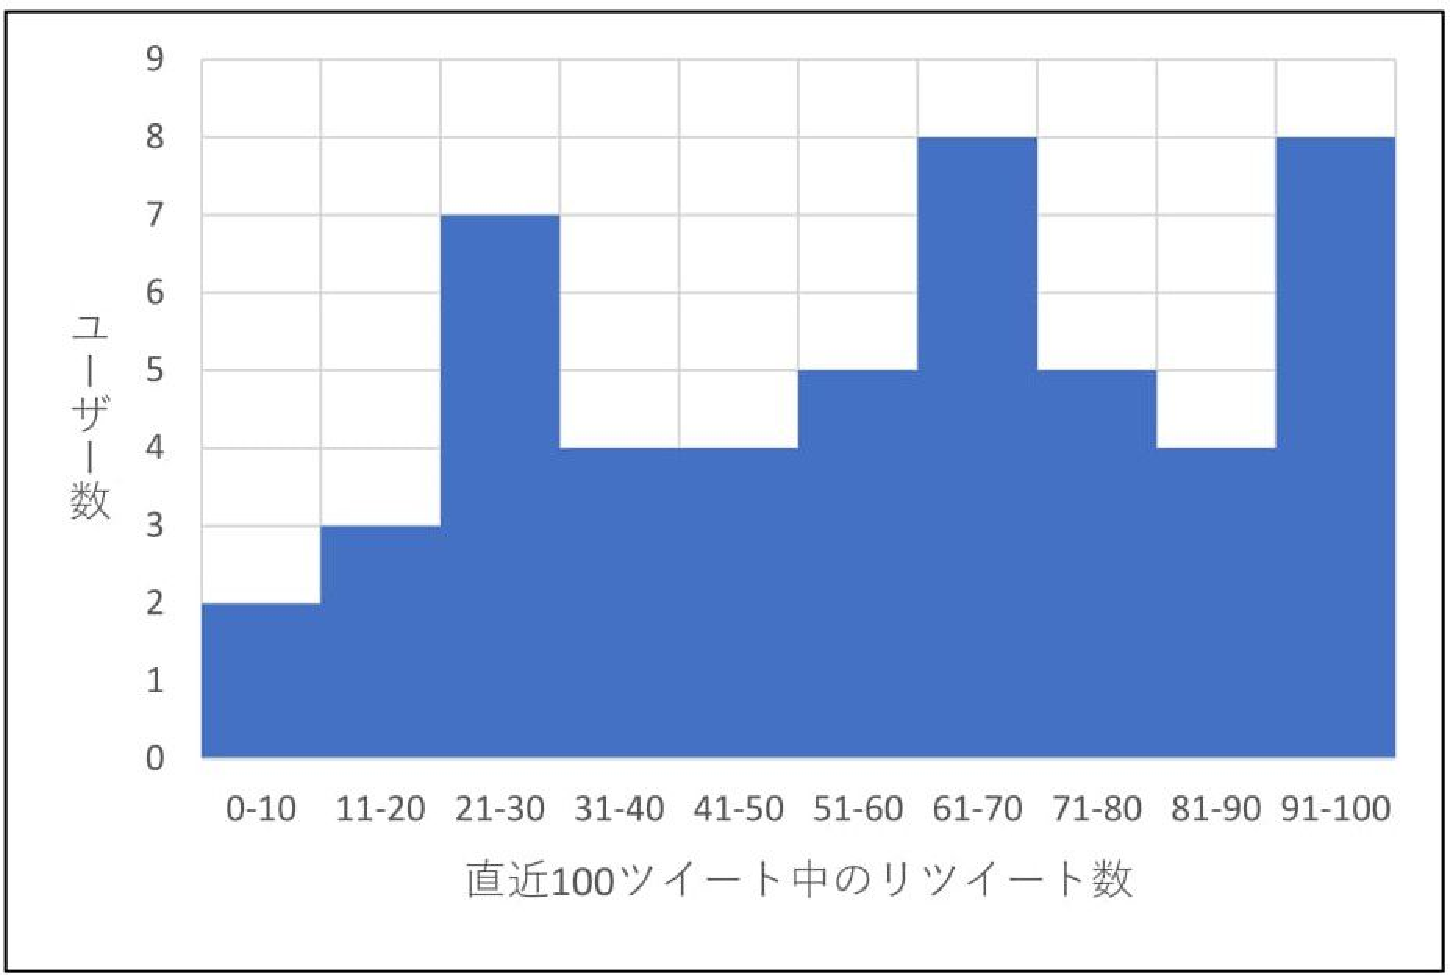
\includegraphics[clip,width=6.0cm,height=3.3cm]{d1.pdf}
\caption{デマツイート1についての結果}
\label{ヒストグラム1}
\end{figure}

\begin{figure}[htbp]
\centering
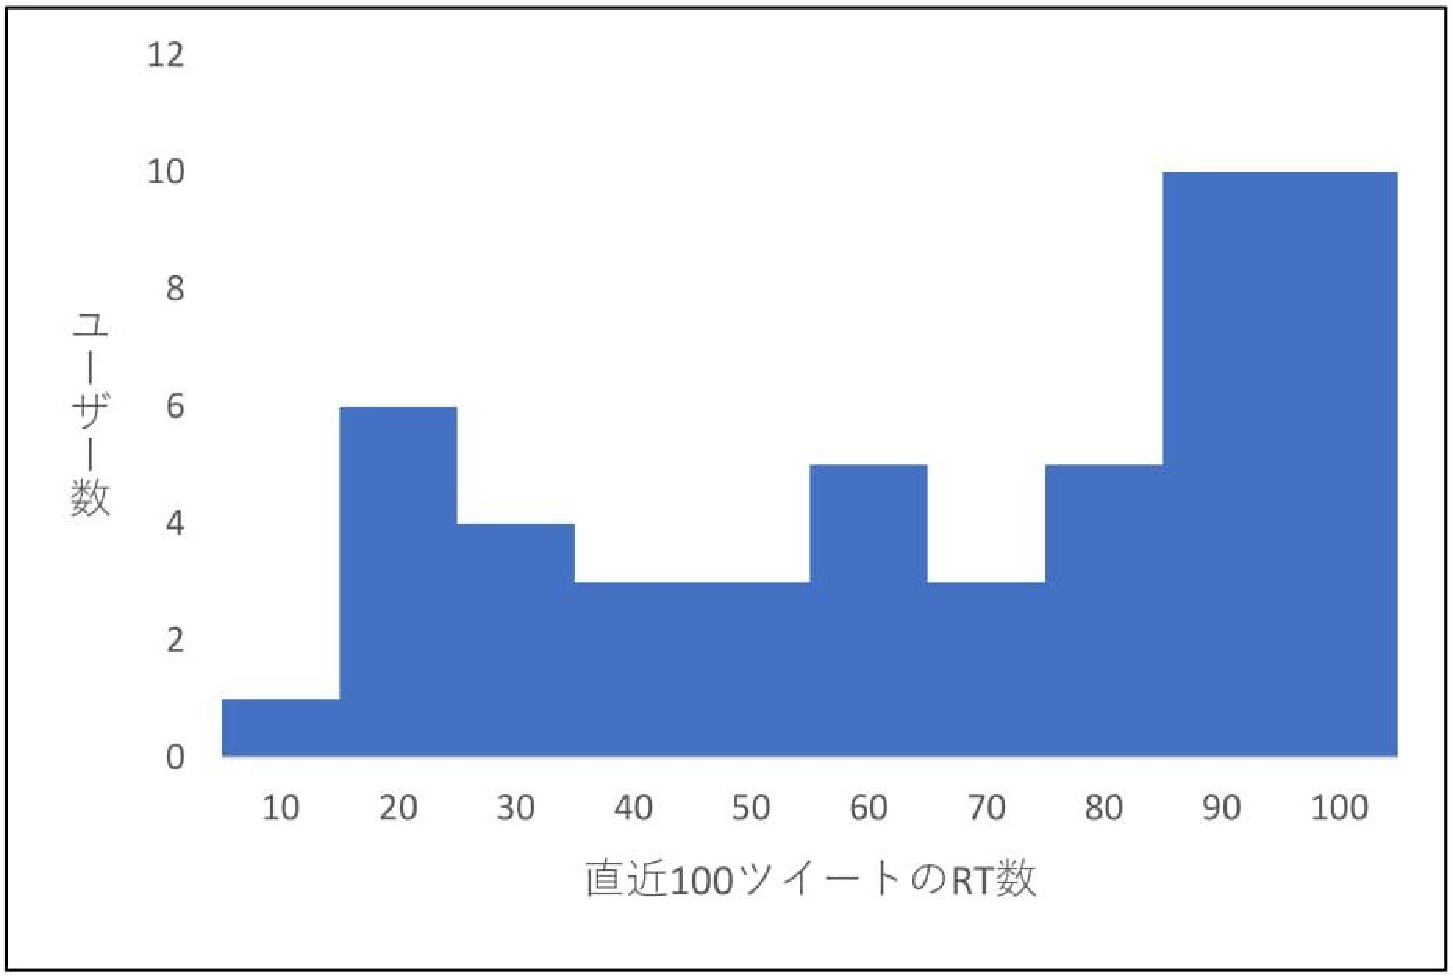
\includegraphics[clip,width=6.0cm,height=3.3cm]{d2.pdf}
\caption{デマツイート2についての結果}
\label{ヒストグラム2}
\end{figure}

\begin{figure}[htbp]
\centering
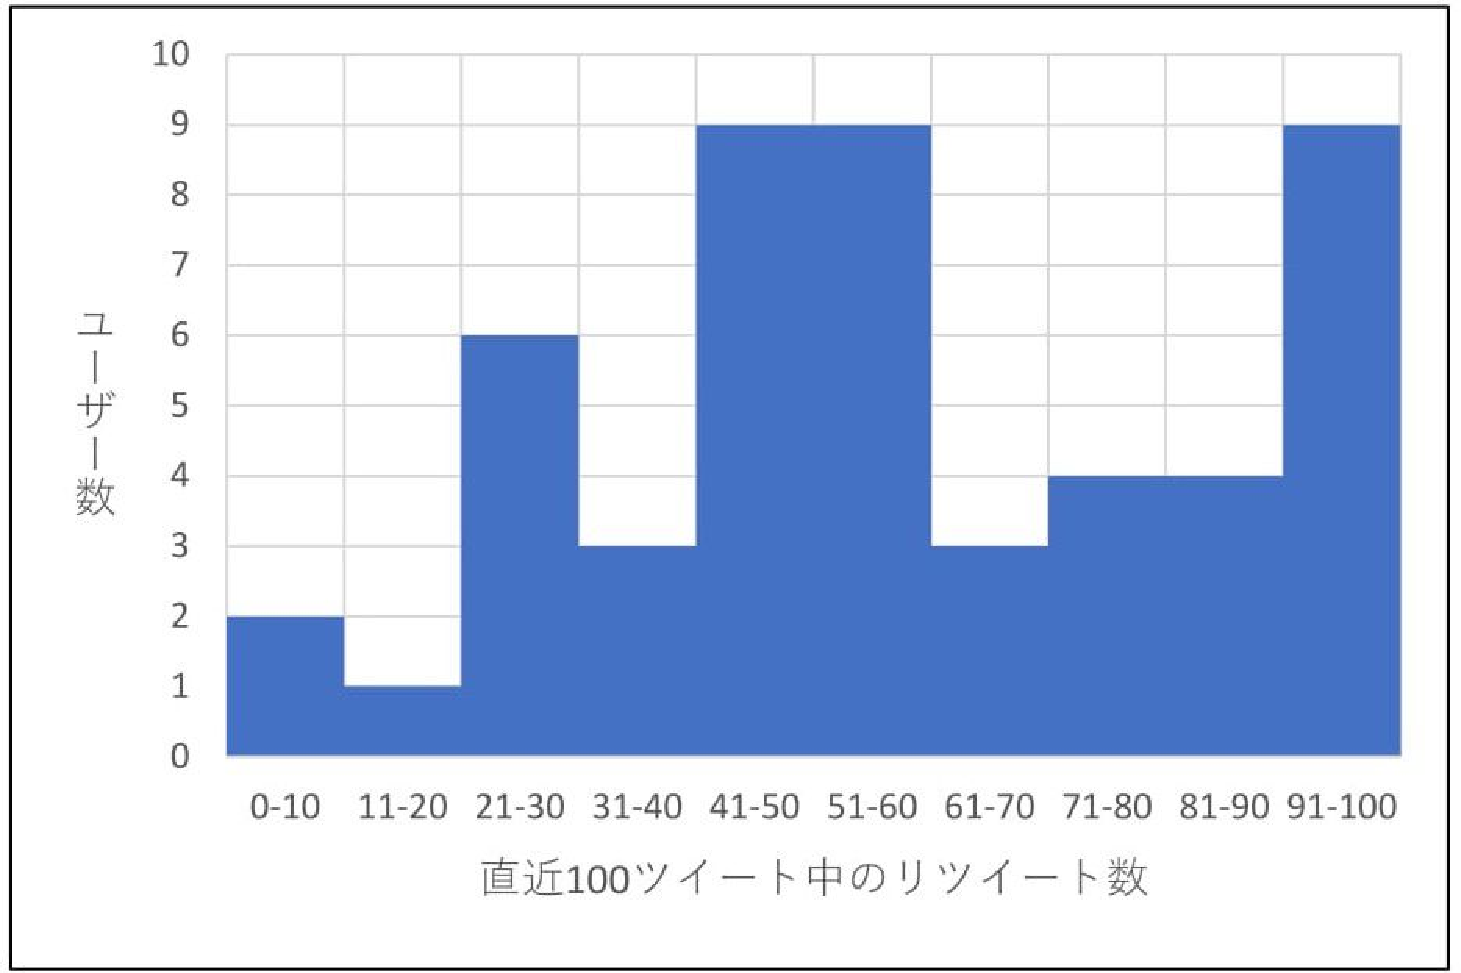
\includegraphics[clip,width=6.0cm,height=3.3cm]{d3.pdf}
\caption{デマツイート3についての結果}
\label{ヒストグラム3}
\end{figure}

\begin{figure}[htbp]
\centering
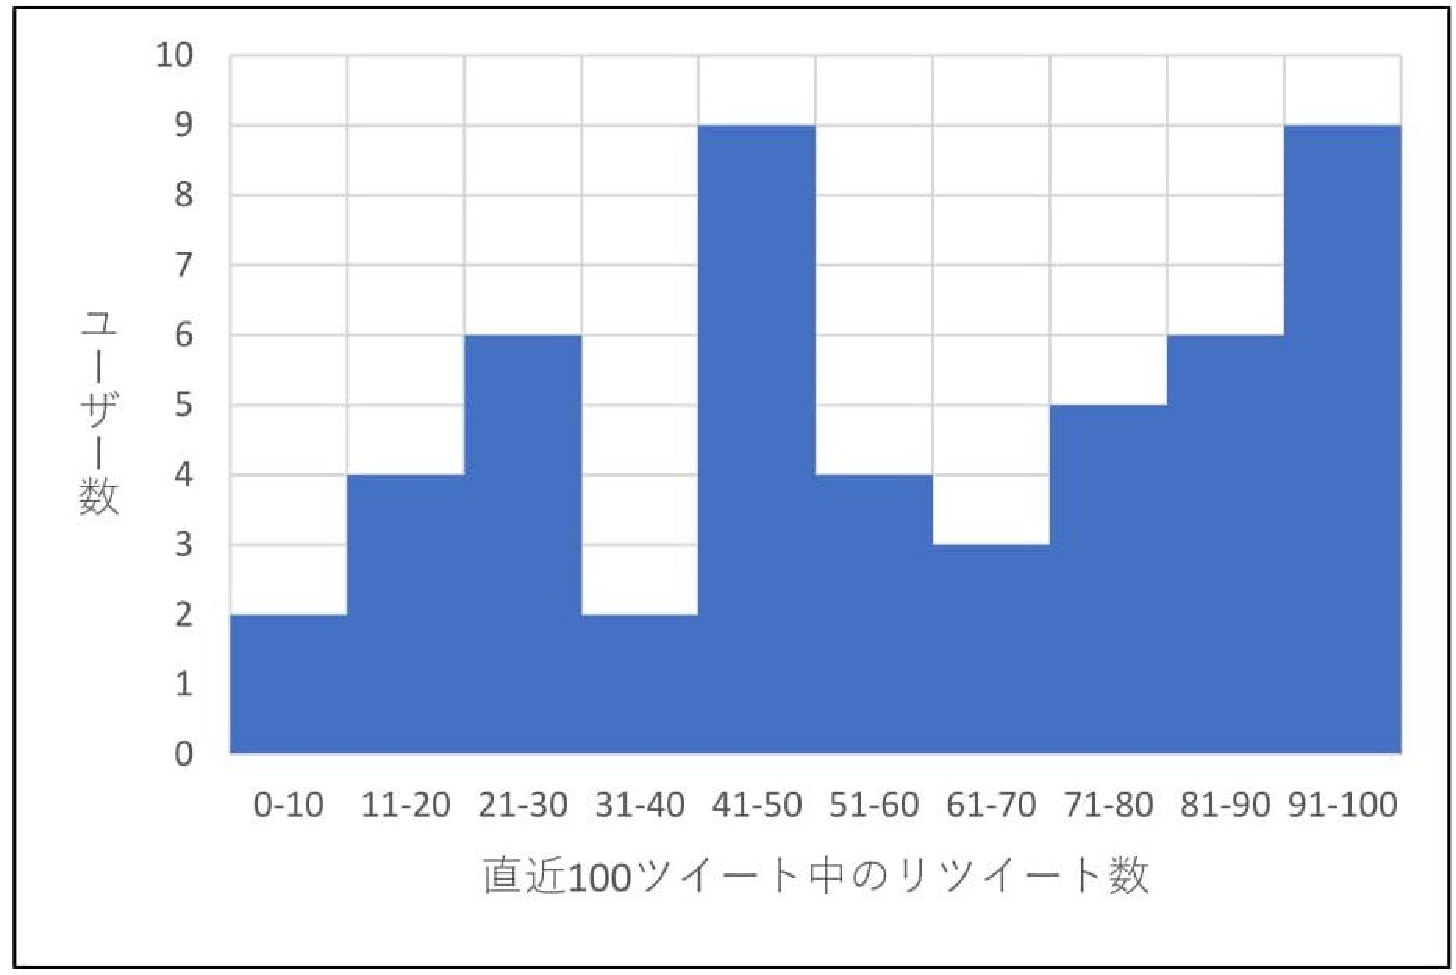
\includegraphics[clip,width=6.0cm,height=3.3cm]{d4.pdf}
\caption{デマツイート4についての結果}
\label{ヒストグラム4}
\end{figure}

\section{考察}
デマを拡散するようなユーザに共通する特徴として,リツイート数に着目しランダムサンプリングしたユーザーとデマツイートをリツイートしたユーザーで直近100リツイート内のリツイート数を調査した結果,大きく数値が異なった.この結果からデマを拡散するようなユーザーはリツイート機能を多用する傾向にあり,ツイート内容の真偽を確かめる前にリツイートをし,デマ拡散者の一員となっていると考えられる.

自分がデマ拡散者にならない為の手段として,デマ拡散ユーザーリストにあるユーザーと,リツイートの多いユーザーを排除することが有効だと考えられる.

\section{結論}
本研究では,デマが拡散されることを防ぐために,デマツイートをリツイートしているユーザーの特徴抽出としてリツイート数の調査を行った.その結果,デマツイートを拡散するユーザーの特徴として,ツイートに占めるリツイートの割合が高いことが確認できた.このような知識を活用することで,Twitterを閲覧する際に,デマツイートを真に受けて拡散してしまうリスクを下げられることが期待できる.
\bibliographystyle{junsrt}
\bibliography{biblio}%「biblio.bib」というファイルが必要.

\end{document}